\documentclass[10pt]{article}
\usepackage[letterpaper,margin=0.9in]{geometry}
\usepackage[T1]{fontenc}
\usepackage{mathptmx}
\usepackage[scaled=0.9]{helvet}
\usepackage{amsmath,graphicx,booktabs,threeparttable,array,tabularx,multirow,makecell,ragged2e,textcomp,url}
\usepackage[table]{xcolor}
\usepackage[font=small,labelfont=bf,labelsep=period]{caption}
\usepackage{cite}
\usepackage{float}
\usepackage{titlesec}
\titleformat*{\section}{\normalsize\bfseries\sffamily}
\titlespacing*{\section}{0pt}{10pt}{4pt}
\definecolor{rowgray}{HTML}{F3F2EF}
\newcommand{\RR}{R\textsuperscript{2}}
\newcommand{\mgdl}{mg/dL}
\renewcommand{\thetable}{S\arabic{table}}
\renewcommand{\thefigure}{S\arabic{figure}}
\renewcommand{\arraystretch}{1.12}
\begin{document}
\begin{center}
{\Large\bfseries\sffamily Supplementary Material}\\[6pt]
{\large Reassessing Photoplethysmography-Based Blood Glucose Estimation: Patient-Independent Validation, Optical Modeling, and Embedded Implementation}\\[6pt]
Mohammad Ghamari, Milan Chhetri, Souvik Kundu, Khalil Alipour, and Bahram Tarvirdizadeh
\end{center}
\noindent Tables and figures referred to without the prefix S are those of the main article. References cited here are listed at the end of this document.

\begin{figure}[H]
\centering
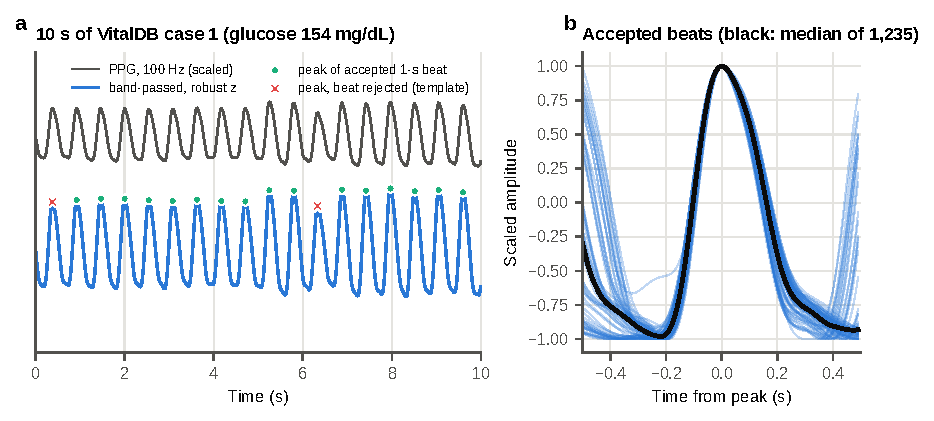
\includegraphics[width=\linewidth]{figs/fig_signal.pdf}
\caption{Preprocessing on real data: the 16-min finger PPG window around the first glucose draw of VitalDB case 1 (154~\mgdl{}), decimated to 100~Hz. (a) Ten seconds of this window (samples 9,500 to 10,500): the PPG and the band-passed, robust z-scored signal with the detected peaks. Green peaks are the centers of accepted 1-s beats; the two red peaks were rejected by the template check (cosine similarity to the mean beat below 0.85). Over the whole window 1,352 peaks were detected and 1,235 beats accepted (91\%). (b) Sixty accepted beats drawn at random from the window, each scaled to $[-1,1]$, and the median of all 1,235.}
\label{fig:signal}
\end{figure}

\begin{table}[H]
\centering\small
\caption{Origin of the optical parameters used in the simulation.}
\label{tab:sources}
\begin{tabularx}{\linewidth}{@{}>{\RaggedRight}p{0.22\linewidth}>{\RaggedRight}X>{\RaggedRight}p{0.2\linewidth}@{}}
\toprule
Parameter & Value and basis & Source \\
\midrule
Glucose scattering coefficient & $\partial\mu_s/\mu_s=-0.29\%$ per mmol/L ($\partial\mu_s/\partial C_g\approx-0.041$~mm$^{-1}$ per mmol/L), measured in 25 oral glucose tolerance tests at 1314~nm and extended over 1000 to 1700~nm with Mie theory & Ge et al.~\cite{ge2024} \\
Independent estimate & $-0.22\%$ per mmol/L near 1300~nm (optical coherence tomography in animals), as cited by Ge et al. & Larin et al.~\cite{larin2003} \\
Geometry & Three layers (0.1 / 1.0 / 10~mm), 0.2~mm glass window, detector rings at 1.7 to 2.9~mm; our model reproduces this geometry & Ge et al.~\cite{ge2024} \\
Glucose absorption, 1000 to 1700~nm & $\partial\mu_a/\partial C_g$ spectrum used by Ge et al. & Ge et al.~\cite{ge2024}; Amerov et al.~\cite{amerov2004} \\
Glucose bands below 1000~nm & CH band near 910~nm; OH bands at 960 and 985~nm change with temperature in the same way as with sugar concentration & Golic et al.~\cite{golic2003} \\
Skin layers, 1000 to 1700~nm & Absorption and reduced scattering spectra of epidermis, dermis and subcutaneous fat, digitized & Iino et al.~\cite{iino2003} \\
Skin layers, 660 to 1000~nm & $\mu_a$ from volume fractions of blood (with saturation), water, fat and melanosomes plus a layer baseline; $\mu_a$ of melanosomes $1.7\times10^{11}\lambda^{-3.48}$~mm$^{-1}$ ($\lambda$ in nm); $\mu_s' = a(\lambda/500\,\mathrm{nm})^{-b}$ with $(a,b)$ = (6.87, 1.161), (4.53, 1.292) and (1.84, 0.672)~mm$^{-1}$ for epidermis, dermis and fat; compared with measured spectra~\cite{simpson1998,shimojo2020} & Jacques~\cite{jacques2013}; Bosschaart et al.~\cite{bosschaart2014} \\
Alternative model, 600 to 1700~nm & Composition-based $\mu_a$ of all layers; $\mu_s'$ measured ex vivo, power-law fit above 1330~nm; $g$ held at 0.91 above 1000~nm; subcutaneous composition; glucose molar absorptivity at 660 and 940~nm & Salomatina et al.~\cite{salomatina2006}; van Gemert et al.~\cite{vangemert1989}; Ganesan et al.~\cite{ganesan2016}; Haque et al.~\cite{haque2021} \\
Conventions & Absorbance $A=-\ln R$ (natural logarithm); glucose sensitivities per mmol/L (1~mmol/L = 18~\mgdl{}) & -- \\
Water absorption & Liquid water at 25~\textdegree C (reported run); Kou et al. in the earlier 1000--1700~nm run, with the same results & Segelstein~\cite{segelstein1981}; Kou et al.~\cite{kou1993} \\
\bottomrule
\end{tabularx}
\end{table}

\begin{table}[H]
\centering\footnotesize\setlength{\tabcolsep}{2.6pt}
\begin{threeparttable}
\caption{Robustness of the deep-network results to the training seed and to two training settings (per-reading scores on VitalDB, fixed folds). Seed rows give mean $\pm$ SD across runs.}
\label{tab:robust}
\begin{tabular}{@{}llcccccc@{}}
\toprule
Model & Split & Runs & \makecell{RMSE\\(\mgdl{})} & \RR{} & Pearson $r$ & \makecell{SD of est.\\(\mgdl{})} & \makecell{Clarke\\A (\%)} \\
\midrule
ResNet34-1D, 1-s beats & Segment & 2 seeds & 31.53 $\pm$ 0.23 & 0.221 $\pm$ 0.011 & 0.563 $\pm$ 0.030 & 9.2 $\pm$ 1.6 & 57.2 $\pm$ 1.0 \\
ResNet34-1D, 1-s beats & Person & 3 seeds & 34.90 $\pm$ 0.06 & 0.046 $\pm$ 0.003 & 0.229 $\pm$ 0.002 & 5.3 $\pm$ 0.7 & 54.4 $\pm$ 0.3 \\
TinyCNN, 1-s beats & Person & 5 seeds & 34.67 $\pm$ 0.06 & 0.058 $\pm$ 0.003 & 0.245 $\pm$ 0.008 & 7.6 $\pm$ 0.2 & 55.4 $\pm$ 0.3 \\
\midrule
ResNet34-1D, lr $3\times10^{-4}$ & Person & 1 & 34.87 & 0.047 & 0.234 & 5.3 & 54.3 \\
ResNet34-1D, 96 beats per reading & Person & 1 & 34.98 & 0.042 & 0.221 & 4.9 & 53.7 \\
\midrule
Age, sex, BMI (ridge) & Person & -- & 35.0 & 0.041 & -- & -- & 54.4 \\
\bottomrule
\end{tabular}
\begin{tablenotes}\footnotesize
\item Seed runs include the original run of Table~4 (seed 42) plus seeds 1--4 (TinyCNN), 1--2 (ResNet34-1D, person split) or 1 (ResNet34-1D, segment-level split). lr: learning rate. The variants use seed 42 and otherwise the settings of Table~3. SD of estimates: spread of the per-reading predictions; laboratory SD 35.7~\mgdl{}.
\end{tablenotes}
\end{threeparttable}
\end{table}

\begin{table}[H]
\centering\small
\caption{PPG computed from the centered window or only from signal before the draw (person-level 5-fold). PPG gain: paired change in RMSE against the same model without PPG, $\Delta\mathrm{RMSE}=\mathrm{RMSE}_{\mathrm{with\ PPG}}-\mathrm{RMSE}_{\mathrm{without\ PPG}}$; a negative value means that PPG improves accuracy. The centered-window rows are the models of Tables~6 and 8.}
\label{tab:causal}
\begin{tabular}{@{}llccc@{}}
\toprule
Setting & PPG window & RMSE (\mgdl{}) & \RR{} & PPG gain [95\% CI] \\
\midrule
No calibration & none (clinical + time) & 32.93 & 0.150 & -- \\
(7,224 readings) & centered $\pm$8~min & 31.82 & 0.207 & $-1.11$ [$-1.50$, $-0.74$] \\
& 8~min before & 32.12 & 0.192 & $-0.81$ [$-1.17$, $-0.45$] \\
& 2~min before & 32.09 & 0.193 & $-0.83$ [$-1.23$, $-0.40$] \\
& 1~min before & 32.03 & 0.196 & $-0.90$ [$-1.26$, $-0.50$] \\
\midrule
One calibration value & none (calibration + clinical + time) & 32.97 & 0.228 & -- \\
(4,233 readings) & centered $\pm$8~min & 31.25 & 0.306 & $-1.72$ [$-2.74$, $-0.84$] \\
& 8~min before & 31.43 & 0.298 & $-1.53$ [$-2.73$, $-0.56$] \\
& 2~min before & 31.34 & 0.302 & $-1.63$ [$-3.14$, $-0.53$] \\
& 1~min before & 31.40 & 0.299 & $-1.57$ [$-3.03$, $-0.57$] \\
\bottomrule
\end{tabular}
\end{table}

\begin{figure}[H]
\centering
\includegraphics[width=\linewidth]{figs/fig_ba.pdf}
\caption{Bland--Altman plots, one point per reading: (a) ResNet34-1D with a person-level split, (b) clinical context, time since anesthesia and PPG features, (c) the calibrated model with all signals. Solid line: mean difference (bias); dashed lines: 95\% limits of agreement. The annotated slopes were obtained by regressing the difference (estimate $-$ laboratory) on the laboratory reference value, not on the mean shown on the horizontal axis; they measure regression toward the mean ($-1$ for a constant estimate, 0 for no proportional error).}
\label{fig:ba}
\end{figure}

\begin{table}[H]
\centering\footnotesize\setlength{\tabcolsep}{3.2pt}
\begin{threeparttable}
\caption{Accuracy by subgroup (person-level 5-fold): RMSE (\mgdl{}) and bias (estimate $-$ laboratory, \mgdl{}).}
\label{tab:subgroups}
\begin{tabular}{@{}llcccccccc@{}}
\toprule
& & \multicolumn{2}{c}{Training-set mean} & \multicolumn{2}{c}{ResNet34-1D} & \multicolumn{2}{c}{Clinical + time + PPG} & \multicolumn{2}{c}{Calibrated, all signals} \\
\cmidrule(lr){3-4}\cmidrule(lr){5-6}\cmidrule(lr){7-8}\cmidrule(l){9-10}
Subgroup & Readings\tnote{a} & RMSE & Bias & RMSE & Bias & RMSE & Bias & RMSE & Bias \\
\midrule
All readings & 7,224 / 4,233 & 35.7 & 0 & 35.0 & $-$1 & 31.8 & 0 & 30.8 & 0 \\
No diabetes & 6,271 / 3,643 & 33.0 & $+$5 & 32.2 & $+$4 & 30.6 & 0 & 30.3 & $+$1 \\
Diabetes & 953 / 590 & 50.3 & $-$30 & 49.4 & $-$30 & 39.0 & $-$1 & 33.7 & $-$4 \\
Below 70~\mgdl{} & 102 / 58 & 59.2 & $+$59 & 58.0 & $+$57 & 51.3 & $+$49 & 62.4 & $+$44 \\
70 to 180~\mgdl{} & 6,661 / 3,800 & 25.2 & $+$6 & 24.6 & $+$5 & 23.3 & $+$4 & 24.5 & $+$4 \\
Above 180~\mgdl{} & 461 / 375 & 100.2 & $-$93 & 98.2 & $-$91 & 86.4 & $-$74 & 63.6 & $-$44 \\
\bottomrule
\end{tabular}
\begin{tablenotes}\footnotesize
\item[a] Readings without / with calibration (the calibrated model scores only readings after a patient's first). Diabetes: pre-operative diabetes in the VitalDB case table (363 patients). Below 70~\mgdl{}: 102 readings from 75 patients without calibration.
\end{tablenotes}
\end{threeparttable}
\end{table}

\begin{table}[H]
\centering\footnotesize\setlength{\tabcolsep}{3.5pt}
\caption{MUST, matched comparison on the 48 recordings (22 people) usable by every model; all models trained on VitalDB. $\Delta\mathrm{RMSE}=\mathrm{RMSE}_{\mathrm{model}}-\mathrm{RMSE}_{\mathrm{constant}}$; a positive value means the model is less accurate than the constant prediction.}
\label{tab:must_matched}
\begin{tabular}{@{}lcccc@{}}
\toprule
Model & RMSE (\mgdl{}) [95\% CI] & MARD (\%) & Pearson $r$ & $\Delta$RMSE vs constant [95\% CI] \\
\midrule
PPG features (GBM) & 23.3 [17.2, 29.4] & 14.8 & $-0.01$ & $+2.6$ [$-1.0$, $+6.9$] \\
PPG features + age, sex, BMI (GBM) & 22.4 [16.2, 28.3] & 13.7 & 0.17 & $+1.6$ [$-2.4$, $+4.9$] \\
Age, sex, BMI (GBM) & 21.8 [15.5, 28.6] & 12.7 & 0.33 & $+1.0$ [$-3.6$, $+5.0$] \\
ResNet34-1D, person split & 21.2 [16.4, 26.1] & 14.9 & $-0.22$ & $+0.4$ [$-0.2$, $+1.0$] \\
TinyCNN, person split & 21.6 [17.5, 25.8] & 15.8 & $-0.03$ & $+0.9$ [$-0.2$, $+2.1$] \\
Constant: VitalDB training mean & 20.7 [16.2, 25.6] & 14.7 & -- & -- \\
\bottomrule
\end{tabular}
\end{table}

\begin{table}[H]
\centering\small
\begin{threeparttable}
\caption{Sensitivity of the optical results to the tissue model: best glucose-equivalent error (\mgdl{}).}
\label{tab:tissue}
\setlength{\tabcolsep}{4pt}
\begin{tabular}{@{}lcccc@{}}
\toprule
& & & \multicolumn{2}{c}{Continuous, glucose also in fat} \\
\cmidrule(l){4-5}
Configuration & \makecell{Main model\\(Table~12)} & \makecell{Continuous\\model} & \makecell{water-\\weighted} & \makecell{full\\strength} \\
\midrule
Single wavelength, best channel & 71 & 73 & 89 & 68 \\
Oximeter wavelengths, 660 / 940~nm & 82 / 84 & 87 / 91 & 102 / 129 & 136 / 114 \\
Glucose absorption only, best channel & 790 & 790 & 750 & 625 \\
Pulsatile channel below 1000~nm & no signal\tnote{a} & no usable signal\tnote{b} & no signal\tnote{a} & no signal\tnote{a} \\
Two wavelengths & none & none & none & none \\
Three wavelengths & none & none & $>$1000 & $>$400 \\
Four / five / six wavelengths\tnote{c} & 11 / 11 / 11 & 15 / 13 / 13 & 20 / 19 / 18 & 18 / 17 / 16 \\
All wavelengths (idealized bound) & 4.0 & 5.1 & 5.6 & 4.8 \\
\bottomrule
\end{tabular}
\begin{tablenotes}\footnotesize
\item none: glucose cannot be separated from the confounders. \item[a] Glucose absorption is set to zero below 1000~nm in this configuration, so the pulsatile channel carries no glucose signal there by construction. \item[b] Zero by construction without glucose absorption below 1000~nm; with the weak absorption of Haque et al.~\cite{haque2021} the glucose-equivalent error is about $4.9\times10^5$~\mgdl{} (the signal is not strictly zero, but far too weak to use). The other rows are identical with and without this absorption to the precision shown. \item[c] Best sets of wavelengths at least 30~nm apart; Monte Carlo 95\% intervals within $\pm$1~\mgdl{}.
\end{tablenotes}
\end{threeparttable}
\end{table}

\begin{table}[H]
\centering\small
\begin{threeparttable}
\caption{ESP32-S3 resources and timing for one 60-s window (240~MHz).}
\label{tab:esp}
\begin{tabular}{@{}lrl@{}}
\toprule
Item & Value & Agreement with Python \\
\midrule
Filtering and beat extraction & 274.7 ms & identical beat counts \\
15 device features & 32.7 ms & bit-identical \\
300 trees, calibration-free & 3.1 ms & 0 \mgdl{} \\
300 trees, calibrated & 3.5 ms & 0 \mgdl{} \\
\rowcolor{rowgray} Device model, total (self-test) & 310.6 ms & 0 \mgdl{} \\
Device model, hardware-in-the-loop, median (range), 30 recordings & 304 (253--340) ms & 0 \mgdl{} \\
Per-beat TinyCNN, 84 beats (network 1,271.2 ms) & 1,554.7 ms & $7.6\times10^{-6}$ \mgdl{} \\
\midrule
Flash: firmware + two tree models (8,700 nodes each) & 945 kB & \\
Free heap after start-up (largest block) & 80 kB (30 kB) & \\
\bottomrule
\end{tabular}
\end{threeparttable}
\end{table}

\begin{thebibliography}{99}
\bibitem{ge2024} Q. Ge \emph{et al.}, ``Evaluation and validation on sensitivity of near-infrared diffuse reflectance in non-invasive human blood glucose measurement,'' \emph{Sensors}, vol.~24, no.~18, Art. no.~5879, 2024, doi: 10.3390/s24185879.
\bibitem{larin2003} K. V. Larin, M. Motamedi, T. V. Ashitkov, and R. O. Esenaliev, ``Specificity of noninvasive blood glucose sensing using optical coherence tomography technique: a pilot study,'' \emph{Phys. Med. Biol.}, vol.~48, no.~10, pp.~1371--1390, 2003, doi: 10.1088/0031-9155/48/10/310.
\bibitem{amerov2004} A. K. Amerov, J. Chen, and M. A. Arnold, ``Molar absorptivities of glucose and other biological molecules in aqueous solutions over the first overtone and combination regions of the near-infrared spectrum,'' \emph{Appl. Spectrosc.}, vol.~58, no.~10, pp.~1195--1204, 2004, doi: 10.1366/0003702042336136.
\bibitem{golic2003} M. Golic, K. Walsh, and P. Lawson, ``Short-wavelength near-infrared spectra of sucrose, glucose, and fructose with respect to sugar concentration and temperature,'' \emph{Appl. Spectrosc.}, vol.~57, no.~2, pp.~139--145, 2003.
\bibitem{iino2003} K. Iino, K. Maruo, H. Arimoto, K. Hyodo, T. Nakatani, and Y. Yamada, ``Monte Carlo simulation of near infrared reflectance spectroscopy in the wavelength range from 1000~nm to 1900~nm,'' \emph{Opt. Rev.}, vol.~10, no.~6, pp.~600--606, 2003.
\bibitem{simpson1998} C. R. Simpson, M. Kohl, M. Essenpreis, and M. Cope, ``Near-infrared optical properties of ex vivo human skin and subcutaneous tissues measured using the Monte Carlo inversion technique,'' \emph{Phys. Med. Biol.}, vol.~43, no.~9, pp.~2465--2478, 1998, doi: 10.1088/0031-9155/43/9/003.
\bibitem{shimojo2020} Y. Shimojo, T. Nishimura, H. Hazama, T. Ozawa, and K. Awazu, ``Measurement of absorption and reduced scattering coefficients in Asian human epidermis, dermis, and subcutaneous fat tissues in the 400- to 1100-nm wavelength range for optical penetration depth and energy deposition analysis,'' \emph{J. Biomed. Opt.}, vol.~25, no.~4, Art. no.~045002, 2020, doi: 10.1117/1.JBO.25.4.045002.
\bibitem{jacques2013} S. L. Jacques, ``Optical properties of biological tissues: a review,'' \emph{Phys. Med. Biol.}, vol.~58, no.~11, pp.~R37--R61, 2013, doi: 10.1088/0031-9155/58/11/R37.
\bibitem{bosschaart2014} N. Bosschaart, G. J. Edelman, M. C. G. Aalders, T. G. van Leeuwen, and D. J. Faber, ``A literature review and novel theoretical approach on the optical properties of whole blood,'' \emph{Lasers Med. Sci.}, vol.~29, no.~2, pp.~453--479, 2014, doi: 10.1007/s10103-013-1446-7.
\bibitem{salomatina2006} E. Salomatina, B. Jiang, J. Novak, and A. N. Yaroslavsky, ``Optical properties of normal and cancerous human skin in the visible and near-infrared spectral range,'' \emph{J. Biomed. Opt.}, vol.~11, no.~6, Art. no.~064026, 2006, doi: 10.1117/1.2398928.
\bibitem{vangemert1989} M. J. C. van Gemert, S. L. Jacques, H. J. C. M. Sterenborg, and W. M. Star, ``Skin optics,'' \emph{IEEE Trans. Biomed. Eng.}, vol.~36, no.~12, pp.~1146--1154, 1989, doi: 10.1109/10.42108.
\bibitem{ganesan2016} G. Ganesan \emph{et al.}, ``Diffuse optical spectroscopic imaging of subcutaneous adipose tissue metabolic changes during weight loss,'' \emph{Int. J. Obes.}, vol.~40, no.~8, pp.~1292--1300, 2016, doi: 10.1038/ijo.2016.43.
\bibitem{haque2021} C. A. Haque, S. Hossain, T.-H. Kwon, and K.-D. Kim, ``Noninvasive in vivo estimation of blood-glucose concentration by Monte Carlo simulation,'' \emph{Sensors}, vol.~21, no.~14, Art. no.~4918, 2021, doi: 10.3390/s21144918.
\bibitem{segelstein1981} D. J. Segelstein, ``The complex refractive index of water,'' M.S. thesis, Univ. Missouri--Kansas City, Kansas City, MO, USA, 1981.
\bibitem{kou1993} L. Kou, D. Labrie, and P. Chylek, ``Refractive indices of water and ice in the 0.65- to 2.5-$\mu$m spectral range,'' \emph{Appl. Opt.}, vol.~32, no.~19, pp.~3531--3540, 1993, doi: 10.1364/AO.32.003531.
\end{thebibliography}
\end{document}
